\documentclass[10pt]{article} % Font size - 10pt, 11pt or 12pt

\usepackage[hmargin=1.25cm, vmargin=1.5cm]{geometry} % Document margins

\usepackage{marvosym} % Required for symbols in the colored box
\usepackage{ifsym} % Required for symbols in the colored box

\usepackage[usenames,dvipsnames]{xcolor} % Allows the definition of hex colors

% Fonts and tweaks for XeLaTeX
\usepackage{fontspec,xltxtra,xunicode}
\defaultfontfeatures{Mapping=tex-text}
%\setmonofont[Scale=MatchLowercase]{Andale Mono}

% Colors for links, text and headings
\usepackage{hyperref}
\definecolor{linkcolor}{HTML}{506266} % Blue-gray color for links
\definecolor{shade}{HTML}{F5DD9D} % Peach color for the contact information box
\definecolor{text1}{HTML}{2b2b2b} % Main document font color, off-black
\definecolor{headings}{HTML}{701112} % Dark red color for headings
% Other color palettes: shade=B9D7D9 and linkcolor=A40000; shade=D4D7FE and linkcolor=FF0080

\hypersetup{colorlinks,breaklinks, urlcolor=linkcolor, linkcolor=linkcolor} % Set up links and colors

\usepackage{fancyhdr}
\usepackage{physics}
\usepackage{amssymb}
\pagestyle{fancy}
\fancyhf{}
% Headers and footers can be added with the \lhead{} \rhead{} \lfoot{} \rfoot{} commands
% Example footer:
%\rfoot{\color{headings} {\sffamily Last update: \today}. Typeset with Xe\LaTeX}

\renewcommand{\headrulewidth}{0pt} % Get rid of the default rule in the header

\usepackage{titlesec} % Allows creating custom \section's

% Format of the section titles
\titleformat{\section}{\color{headings}
\scshape\Large\raggedright}{}{0em}{}[\color{black}\titlerule]

\title{Solid State Assignment One}
\author{Elliott Capek}
\titlespacing{\section}{0pt}{0pt}{5pt} % Spacing around titles

\begin{document}

\maketitle{}

\section{Problem 1: D functions as linear combinations}
For each of the five d-orbitals wavefunctions, create a 3D plot of the angular wave and express
the angular wave as a linear combination of spherical harmonics, like so:

\begin{align*}
  d_{x^2-y^2} &= a_{00}Y_{00} + a_{1-1}Y_{1-1} + a_{10}Y_{10} + a_{11}Y_{11} + a_{20}Y_{20} + ...\\
\end{align*}

\subsection{d_{xy}}
\begin{align*}
  d_{xy} &= \left(\frac{15}{4\pi}\right)^{1/2}\frac{xy}{r^2}\\
\end{align*}

%% \begin{figure}[h!]
%%   \caption{\textbf{}
%%   \centering
%%   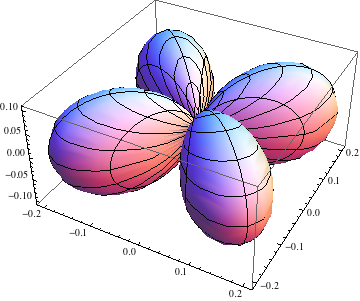
\includegraphics[width=0.5\textwidth]{../figures/dxy.png}
%%   \label{fig:dxy}
%% \end{figure}

\subsection{d_{xy}}
\begin{align*}
  d_{xy} &= \left(\frac{15}{4\pi}\right)^{1/2}\frac{xy}{r^2}\\
\end{align*}

%% \begin{figure}[h!]
%%   \caption{\textbf{}
%%   \centering
%%   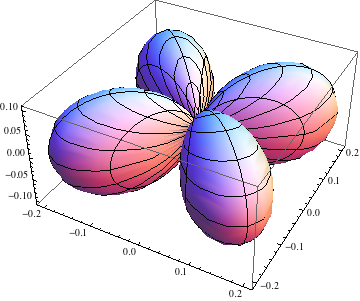
\includegraphics[width=0.5\textwidth]{../figures/dxy.png}
%%   \label{fig:dxy}
%% \end{figure}

\subsection{d_{xy}}
\begin{align*}
  d_{xy} &= \left(\frac{15}{4\pi}\right)^{1/2}\frac{xy}{r^2}\\
\end{align*}

%% \begin{figure}[h!]
%%   \caption{\textbf{}
%%   \centering
%%   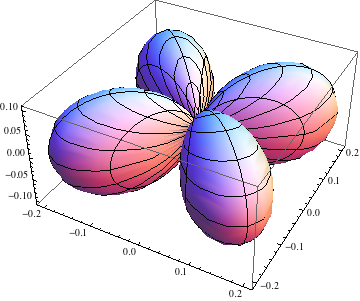
\includegraphics[width=0.5\textwidth]{../figures/dxy.png}
%%   \label{fig:dxy}
%% \end{figure}

\subsection{d_{xy}}
\begin{align*}
  d_{xy} &= \left(\frac{15}{4\pi}\right)^{1/2}\frac{xy}{r^2}\\
\end{align*}

%% \begin{figure}[h!]
%%   \caption{\textbf{}
%%   \centering
%%   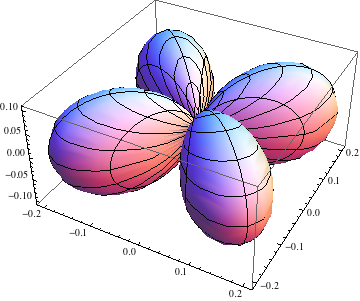
\includegraphics[width=0.5\textwidth]{../figures/dxy.png}
%%   \label{fig:dxy}
%% \end{figure}

\subsection{d_{xy}}
\begin{align*}
  d_{xy} &= \left(\frac{15}{4\pi}\right)^{1/2}\frac{xy}{r^2}\\
\end{align*}

%% \begin{figure}[h!]
%%   \caption{\textbf{}
%%   \centering
%%   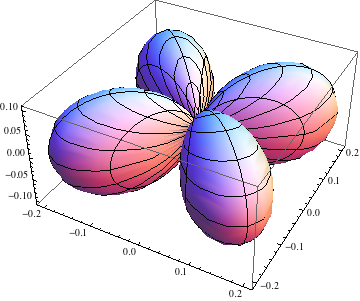
\includegraphics[width=0.5\textwidth]{../figures/dxy.png}
%%   \label{fig:dxy}
%% \end{figure}

\end{document}
